%
% File coling2020.tex
%
% Contact: feiliu@cs.ucf.edu & liang.huang.sh@gmail.com
%% Based on the style files for COLING-2018, which were, in turn,
%% Based on the style files for COLING-2016, which were, in turn,
%% Based on the style files for COLING-2014, which were, in turn,
%% Based on the style files for ACL-2014, which were, in turn,
%% Based on the style files for ACL-2013, which were, in turn,
%% Based on the style files for ACL-2012, which were, in turn,
%% based on the style files for ACL-2011, which were, in turn, 
%% based on the style files for ACL-2010, which were, in turn, 
%% based on the style files for ACL-IJCNLP-2009, which were, in turn,
%% based on the style files for EACL-2009 and IJCNLP-2008...

%% Based on the style files for EACL 2006 by 
%%e.agirre@ehu.es or Sergi.Balari@uab.es
%% and that of ACL 08 by Joakim Nivre and Noah Smith

\documentclass[11pt]{article}
\usepackage{coling2020}
\usepackage{times}
\usepackage{url}
\usepackage{latexsym}
\renewcommand{\UrlFont}{\ttfamily\small}
\usepackage{graphicx}
\usepackage{tikz}
\usepackage{pgfplots}
\usepackage{subcaption}
\usepackage{url}
\usepackage{booktabs}
\usepackage{microtype}

% New command added by Hoang
\newcommand\BibTeX{B\textsc{ib}\TeX}
\newcommand{\argmax}[1]{\underset{#1}{\operatorname{arg}\,\operatorname{max}}\;}
\newcommand\footnoteref[1]{\protected@xdef\@thefnmark{\ref{#1}}\@footnotemark}
\newcommand{\todo}[1]{\textcolor{red}{TODO: #1}}
\newcommand{\comment}[1]{\textcolor{blue}{In Progress: #1}}



%\setlength\titlebox{5cm}
%\colingfinalcopy % Uncomment this line for the final submission

% You can expand the titlebox if you need extra space
% to show all the authors. Please do not make the titlebox
% smaller than 5cm (the original size); we will check this
% in the camera-ready version and ask you to change it back.


\title{AutoSMeT: The Autocompletion Application for Simplifying Medical Text}

\author{First Author \\
  Affiliation / Address line 1 \\
  Affiliation / Address line 2 \\
  Affiliation / Address line 3 \\
  {\tt email@domain} \\\And
  Second Author \\
  Affiliation / Address line 1 \\
  Affiliation / Address line 2 \\
  Affiliation / Address line 3 \\
  {\tt email@domain} \\}

\date{}

\begin{document}
\maketitle
\begin{abstract} 
  The goal of text simplification is to transform difficult text into a version that is easier to understand and more broadly accessible.  In some domains, such as healthcare and medicine, fully automated approaches cannot be used since information must be accurately preserved. In this paper, we introduce a first-of-its-kind medical data set that pairs English Wikipedia with Simple English Wikipedia and the application of pretrained language models (LMs) in autocompletion for text simplification in medical domain. Our autocompletion model aims to assist human simplification by suggesting the next word to type when manually simplifying a text. We compare four pre-trained neural LMs (PNLMs) (BERT, RoBERTa, XLNet, and GPT-2) and show how the additional context of the sentence to be simplified can be incorporated to achieve significantly better results (in the range of 9.0\% to 28.8\% absolute improvement). The best model, RoBERTa with context, achieves a word prediction rate of 62.4\% on medical Wikipedia data. With the conducted LM comparison, we introduce the AutoASMet ensemble model that combines the adventanges of four PNLMs and outperforms RoBERTa by 2.1\%.

\end{abstract}

\section{Introduction}

Text simplification (TS) is the process of modifying the words and structure of a text while preserving the content to make the information in the text more broadly accessible \cite{shardlow2014survey}. Most of the researches in text simplification have focused on fully automated \cite{zhu10,coster2011learning,xu2016optimizing,zhang2017sentence,nishihara2019controllable}. However, in some domains, e.g., healthcare and medicine, using fully-automated text simplifications is not appropriate because it is critically required that information is preserved fully and correctly during the simplification process. \cite{shardlow2019neural} shows that fully-automated text simplification models only simplify 5.8\% of clinical sentences while preserving critical information. These models tend to obmit information in clinical text, which is critical to both doctors and patients (approximately 30\% showed by \cite{shardlow2019neural}). Therefore, instead of fully-automated approaches, support tools such as editors are better suited to generate simplifications with higher efficiently and quality \cite{kloehn2018jmir}.

In this paper, we explore the application of PNLMs to autocompletion models for sentence-level medical text simplification. Given a difficult sentence that a user is trying to simplify and the simplification typed so far, the goal is to correctly suggest the next word to follow what has been typed. Table \ref{tab:example} shows an example of a difficult sentence along with a simplification that the user has typed so far. The autocompletion models will predict the next word to assist in finishing the simplification, in this case a verb like ``take'', which might be continued to a partial simplification of ``take place at the Chapel''. In contrast to most autocomplete applications, in addition to the text that is being typed, our models for text  simplification benefit from additional context of the content being simplified. This unique characterisitic allows autocomplete models to efficiently simplify medical text with high quality while correctly preserving crucial information, which cannot be found in most fully-automated models. The contribution of our work are four-fold:

\begin{table}
    \centering
    \scalebox{0.9}{%
    \begin{tabular}{l l}
    \toprule
    Difficult & The Chapel is actively used as a place of\\
    sentence & worship and also for some concerts and\\
     & college events. \rule[-2ex]{0pt}{0pt} \\ 
    \hline
    Typed &  Concerts and college events $\rule{1cm}{0.15mm}$ \rule{0pt}{3ex} \\
    \bottomrule
    \end{tabular}}
    \caption{An example text simplification autocompletion task.  The user is simplifying the difficult sentence on top and has typed the words on the bottom so far.}
    \label{tab:example}
\end{table}

\noindent {1.} We introduce a first-of-its-kind medical data set that pairs English Wikipedia and Simple Wikipedia, which is automatically extracted from the Simple Wikipedia parallel corpus \cite{kauchak2013improving}. The resulting medical corpus has 3.3k sentence pairs, of which an estimated 2.8k are genuinely medical.

\noindent {2.} We also examine the PNLMs on autocompletion task for sentence simplification and provide an initial analysis based on a number of recent models. We show that the additional context of the difficult sentence can be integrated into these models to improve the quality of the suggestions made.  RoBERTa is the best individual model with 62.4\% accuracy (19.4\% above our base-line).

\noindent {3.} We introduce the AuTS, the ensemble model that combines adventages of recent PNLMs. Our model outperforms the best single PNLM, RoBERTa, by 2.1\%. Further, to our best knowledge, this ensembling approach is novel and suggests a potential improvements on PNLMs for natural language processing (NLP) downstream tasks.

\noindent {4.} Finally, we publish an interface of our autocomplete models, which can be used to simplify medical text in real time.

\section{Related Work}

Autocompletion tools suggest one or more words as the user types that could follow what has been typed so far. Autocompletion has been used in a range of applications including web queries \cite{cai2016survey}, database queries \cite{khoussainova2010snipsuggest}, texting \cite{dunlop2000predictive}, and e-mail composition \cite{dai2019gmail}. Our work is most similar to interactive machine translation tools where a user translating a foreign sentence is given guidance as they type \cite{green-etal-2014-human}.

\section{Approach}

Given a difficult sentence that a user is trying to simplify, $d_1 d_2 ... d_m$, and the simplification typed so far, $s_1 s_2 ... s_i$, the goal of autocompletion model is to suggest word $s_{i+1}$. To evaluate the quality of the different models, we used the first-of-its-kind medical corpus (see section \ref{sec:medical_corpora}) that we extracted from the Simple Wikipedia parallel corpus \cite{kauchak2013improving}, which contains 167K pairs of sentences. Each pair consists of one sentence from English Wikipedia and a corresponding sentence from Simple English Wikipedia. We used 70\% of the sentence pairs for training, 15\% for development, and 15\% for testing. 

To evaluate the models, we calculated how well the models predicted the next word in a test sentence, given the previous words.  A simple test sentence of length $n$, $s_1 s_2 ... s_n$, would result in $n-1$ predictions, i.e., predict $s_2$ given $s_1$, predict $s_3$ given $s_1 s_2$, etc.  For example, Tabel \ref{tab:medexample} shows a difficult sentence from English Wikipedia and the corresponding simplification from the medical Simple English Wikipedia. Given this test example, we generate 19 \todo{AHMAD: please fix the prediction tasks table and add the final number here} prediction tasks, one for each word in the simple sentence after the first word.  Table \ref{fig:testing} shows these six test prediction tasks.  For the context-aware approaches, a coressponding difficult sentence is concatenated as a prefix for each prediction task. We measured the performance of a system using accuracy based on the number of predictions that exactly matched the next word in the corpus.  The test corpus contained 495 sentence pairs resulting in a total of 7969 individual word predictions.

\begin{table}
    \centering
    \scalebox{0.9}{%
    \begin{tabular}{l l}
    \toprule
    Difficult & The Saxons built Banbury on the west \\
    sentence & bank of the River Cherwell. \rule[-2ex]{0pt}{0pt} \\ 
    \hline
    Simple & Banbury is part of the Cherwell district. \rule{0pt}{3ex}\\
    sentence &  \\
    \bottomrule
    \end{tabular}}
    \caption{An example sentence pair from the English Wikipedia corpus.}
    \label{tab:testexample}
\end{table}

\todo{AHMAD: after you finished Medical Corpora part, please fix this table with a medical example.}
\begin{table}
\centering
\scalebox{0.9}{%
\begin{tabular}{ll}
\toprule \textbf{Typed so far} & \textbf{Predict} \\
\midrule
Banbury & is \\
Banbury is & part \\
Banbury is part & of \\
Banbury is part of & the \\
Banbury is part of the & Cherwell \\
Banbury is part of the Cherwell & district \\
\bottomrule
\end{tabular}}
\caption{The resulting prediction tasks that are generated from the example in Table \ref{tab:testexample}.}
\label{fig:testing}
\end{table}

\begin{table}[t]
\centering
\scalebox{0.87}{%
\begin{tabular}{c c c }
\toprule
\textbf {Model} &\textbf{No Context} & \textbf {Context-Aware}\\ 
\midrule
RoBERTa & 56.23\% & \textbf{62.4}\% \\
\midrule
BERT & 53.28\% & 50.43\% \\
\midrule
XLNet & 46.2\% & 45.7\% \\
\midrule
GPT-2 & 23.2\% & 49\% \\
\bottomrule
\end{tabular}}
\caption{Accuracy for the different models on the Wikipedia test corpus of 450 sentence pairs.  Context-aware approaches included the context of the difficult sentence when predicting.} 
\label{tab:results}
\end{table}

In this work, we examined four recent PNLMs that utilize the Transformer network \cite{vaswani2017attention}: BERT \cite{devlin2018bert}, RoBERTa \cite{liu2019roberta}, XLNet \cite{yang2019xlnet}, and GPT-2 \cite{radford2019language} and the AutoASMeT ensemble models, which combines the advantages of the transformer-based models.

\subsection{Transformer-based Language Models}

%Neural language models use neural networks, often with many layers, to predict the likelihood of the next word given the context (and, in some cases, e.g., transformer models, actually predict the next word).  
%Unlike $n$-gram language models which are restricted to a fixed context, neural models use either recurrent neural networks \cite{mikolov2010recurrent}, Transformer networks, or other similar network configurations that build up an encoding of the context of the previous words and are therefore not limited to a fixed context window. 

We examined four PNLMs based on Transformers network: BERT, RoBERTa, XLNet, GPT-2. To apply the models to our autocomplete task, we predict the next word for the input ``$s_1 s_2 ... s_i \mbox{[NEXT]} .$''. For the context-aware version, we concatenate the context of the difficult sentence
``$d_1 d_2 ... d_m. s_1 s_2 ... s_i \mbox{[NEXT]} .$''. This biases the prediction to words related to those found in the encoded context from difficult sentences. We also fine-tuned all four models on general parallel English Wikipedia \cite{kauchak2013improving} and further fine-tuned them on the separate medical training set described in section \ref{sec:medical_corpora}. This two-step fine-tuning helps the models learn the domain knowledge of the text simplification task and the specific language of medical text.

\subsubsection{BERT} 

BERT (Bidirectional Encoder Representations from Transformers) is a method for learning language representations using bidirectional training.BERT has been shown to produce state-of-the-art results in a wide range of generation and classification applications \cite{devlin2018bert}. In this work, we use the base original BERT model pre-trained on the BooksCorpus \cite{zhu2015aligning} and English Wikipedia. We finetuned the pytorch BERT implemented by the huggingface\footnote{\url{https://github.com/huggingface/bert/}}. The BERT fine-tuning was done with a batch-size of 8, 8 epochs, and a learning rate of $5e^{-5}$. Early stopping was used based on the second time a decrease in the accuracy was seen.

\subsubsection{RoBERTa} \comment{HOANG}

RoBERTa is A Robustly Optimized BERT Pretraining Approach. The RoBERTa uses the same model architecture as BERT. However, the differences between RoBERTa and BERT are that RoBERTa does not use Next Sentence Prediction during pre-trainining and RoBERTa uses larger mini-batch size. We used the publicly released base RoBERTa with 125M parameters model \footnote{\url{https://github.com/huggingface/roberta}}. The RoBERTa fine-tuning was done with a batch-size of 8, 8 epochs, and a learning rate of $5e^{-5}$. Early stopping policy was also similar to BERT fine-tuning.

\subsubsection{XLNet}

XLNet is a generalized autoregressive pretraining method. Like BERT, XLNet benefits from bidirectional contexts. However, XLNet does not suffer limitations of BERT because of its autoregressive formulation. In this work, we used publicly available base English XLNet with 110M parameters version implemented in pytorch\footnote{\url{https://github.com/huggingface/xlnet}}. The XLNet fine-tuning was done with a batch-size of 8, 8 epochs, and a learning rate of $5e^{-5}$. Early stopping policy was also similar to BERT fine-tuning.

\subsubsection{GPT-2}

Like BERT, GPT-2 is also based on the Transformer network, however, GPT-2 uses unidirectional left-to-right pretraining process. We use the publicly released model\footnote{\url{https://github.com/openai/gpt-2}}, which has 124M parameters and is trained on web text. The GPT-2 fine-tuning was done with a batch-size of 8, 8 epochs, and a learning rate of $5e^{-5}$. Early stopping policy was also similar to BERT fine-tuning.

\subsection{Ensembling Models}

By combining adventages of four PNLMs, we examined four ensembling approaches and reported their performance in section \ref{sec:results}. Our best ensemling model AutoASMeT, which uses neural trained hypothesis selection mechanism, outperforms the best single PNLM by 2.1\%. 

\subsubsection{Majority Vote}

As shown in section \ref{tab:accuracy-@-n}, PNLMs benefit from the increase in number of suggestions. For this ensembling approach, we take the best 5 suggestions from each model and do a majority count in the pool of combined suggestions. The output of the model is the suggestion with most count. If there is a tie, we randomly select one of them. Due to this randomness, we repeat the experiment for 10 times and report the average performance in table \ref{tab:ensembleResults}.

\subsubsection{4CC} \label{sec:4cc}

The 4CC model is an ensembling approach, which we trained a classifier to pick the most approriate model among four PNLMs, given the next-word prediction task. We trained a neural text classification implemented by huggingface\footnote{\url{https://github.com/huggingface/transformers}} with the training set consists sample similar to table \ref{tab:4ccexample}. Each next-word prediction task is labeled with one of the four options (RoBERTa, BERT, XLNet, GPT-2). This text classification is used as a model selection for our 4CC ensembling model. We designed a scoring system for model selection as follow:
\begin{equation} \label{eq:4cc}
	Score(w, X) = \alpha * P(w|X) + \theta * I (X, S)
\end{equation}
In equation \ref{eq:4cc}, $P(w|X)$ is the model $X$'s confidence on predicted word $w$, $I(X, S)$ is an identity function (which return $1$ if $X = S$ and $0$ otherwise), $S$ is the predicted model from model selector, $\alpha$ and $\theta$ are scoring parmeters.  
At testing time, we pick the highest score and output the word $w$, given a prediction task.  

\begin{table}
    \centering
    \scalebox{1}{%
    \begin{tabular}{l c}
    \toprule
    \textbf{Prediction Task}  & \textbf{Class} \\
    \midrule
    (Difficult sentence). This (MASK) & RoBERTa \\
    (Difficult sentence). This insulin (MASK) & BERT \\
    (Difficult sentence). This insulin tells (MASK) & XLNet \\
    \bottomrule
    \end{tabular}}
    \caption{An example of tranining data for the 4CC model. Class can be one of the four option: RoBERTa, BERT, XLNet, GPT-2}
    \label{tab:4ccexample}
\end{table}

\subsubsection{AutoASMeT}

Because of the strong bias toward RoBERTa in training data for model selection in section \ref{sec:4cc}, we decide to use a multi-label classifier for model selector in the AutoASMeT. This choice of model selector, to our knowledge, is novel to trasnformer-network-based ensembling models. For this choice of classifier, each prediction task is given a sequence of 4 labels with value of 0 and 1. Each label represents one of the four PNLMs. Table \ref{tab:autoasmetexample} shows an example of this dataset. We trained a neural multi-label classifier implemented by huggingface \footnote{\url{https://github.com/huggingface/transformers}} on this training dataset and used it as AutoASMeT's model selector. We designed a scoring system for model selection as follow:
\begin{equation} \label{eq:autoasmet}
	Score(w, X) = \beta * P(w|X) + \sigma * S(X, Ls)
\end{equation}
In equation \ref{eq:autoasmet}, $P(w|X)$ is the model $X$'s confidence on predicted word $w$, $S(X, Ls)$ is a function (which return $0.25$ if model $X$ is in $Ls$ and $0$ otherwise), $Ls$ is the predicted sequence of labels from model selector, $\beta$ and $\sigma$ are scoring parmeters.  
At testing time, we pick the highest score and output the word $w$, given a prediction task.

\begin{table}
    \centering
    \scalebox{1}{%
    \begin{tabular}{l c}
    \toprule
    \textbf{Prediction Task}  & \textbf{Sequence of Labels} \\
    \midrule
    (Difficult sentence). This (MASK) & 1 0 1 1 \\
    (Difficult sentence). This insulin (MASK) & 0 1 0 0 \\
    (Difficult sentence). This insulin tells (MASK) & 1 1 1 1 \\
    \bottomrule
    \end{tabular}}
    \caption{An example of tranining data for the AutoASMeT model. For a prediction task, a sequence of 4 labels is give in the order "RoBERTa BERT XLNet GPT-2". The value of 1 means the model correctly predict the right word, and 0 otherwise.}
    \label{tab:autoasmetexample}
\end{table}

\subsubsection{Upper Bound}

To see how well the AutoASMeT model perform, we examine the upper bound, which is the best performanance any ensemble model can achieve. For the upperbound, as long as at least one model among the four PNLMs correctly predicts the next word, given a predicton task, we mark it as correct for the Upper Bound model. This means that no other possible combination of PNLMs can perform any better.

\section{Medical Parallel Wikipedia Corpus} \label{sec:medical_corpora}\comment{Ahmad is currently working on this}

\todo{AHMAD: can you make this longer and give more details on the corpora creation. Please make sure to include citation from the paper I sent early}
%In this paper, to create the medical corpus, we use the simple parallel Wikipedia corpus by \cite{kauchak2013improving}, which contains 167K pairs of sentences, with one sentence from English Wikipedia and a corresponding sentence from Simple English Wikipedia. Table \ref{tab:testexample} shows an example sentence pair. To extract the medical samples, first, we created a medical dictionary with 269 health-related keywords\footnote{\url{https://figshare.com/articles/List_of_Health_Keywords/1084358}} and 260k medical terms selected from the Unified Medical Language System \cite{bodenreider2004unified}. The UMLS terms were those related to medical semantic types. Second, we extracted sentences from the English Wikipedia corpus using this medical dictionary as follows: if the title and the body of a sentence from Wikipedia normal corpus have 4 matching words with our medical keywords, then that sentence (both normal and simple version) is added to the medical corpus. The resulting medical corpus has 3.3k sentence pairs, of which an estimated 2.8k are genuinely medical. An example of medical sentence pair is shown in Table \ref{tab:medexample}. Table \ref{tab:medsize} shows the corpus size for two corpora. 

\begin{table}
    \centering
    \scalebox{0.9}{%
    \begin{tabular}{l l}
    \toprule
    Difficult & Lowered glucose levels result both in the \\
    sentence  & reduced release of insulin from the beta \\
              & cells and in the reverse conversion of\\
              & glycogen to glucose when glucose levels \\
              & fall.
    \rule[-2ex]{0pt}{0pt} \\ 
    \hline
    Simple & This insulin tells the cells to take up
    \rule{0pt}{3ex}\\
    sentence & glucose from the blood. The glucose is \\
             & used by cells for energy \\
    \bottomrule
    \end{tabular}}
    \caption{An example of sentence pair in Medical Wikipedia parallel corpus.}
    \label{tab:medexample}
\end{table}

\begin{table}
    \centering
    \scalebox{1}{%
    \begin{tabular}{l c}
    \toprule
    \textbf{Domain}  & \textbf{No. Sentence Pairs} \\
    \midrule
    General Domain & 163,700 \\
    Medical Domain & 3,300 \\
    \midrule
    Total & 167,000\\
    \bottomrule
    \end{tabular}}
    \caption{Number of sentence pairs for General Domain and Medical Domain. The two corpora are exclusive.}
    \label{tab:medsize}
\end{table}

\section{Results} \label{sec:results}

We provide the first results on this task using BERT, RoBERTa, XLNet, and GPT-2, with and without context, as well as an no-fine-tuned BERT as a baseline. We provide an initial analysis of model performance and use it to design the AuTS, which is an ensemble model which combines advantages of each PNLM.

\subsection{Experimental setup}



As an additional baseline that does not use context, we trained a trigram language model with Kneser-Ney smoothing using the SRILM toolkit \cite{stolcke2002srilm}.  The model was trainined on the simple sentences from the training portion of the dataset and predicts $s_{i+1}$ as the word with the highest probability given the previous two words, i.e., $argmax_{s_{i+1}}\mbox{ } p(s_{i+1}| s_i s_{i-1})$.



\todo{Add RoBERTa, XLNet, GPT-2 fintuning set up here}

\subsection{Prediction performance}
Table \ref{tab:results} shows the results for the five different variants (trigram model, BERT and GPT-2 with and without context).  Both neural models significantly outperform the trigram language model; they have been trained on larger corpora and have access to more context allowing for better predictions.  Without context, GPT-2 performs slightly better than BERT, with an absolute improvement of 1.7\%.  To put these accuracy numbers in perspective, in an actual autocomplete task, without context, both BERT and GPT-2 would get about every 4th or 5th word/suggestion correct.

With context, the results improve drastically and the accuracy rates double for both models.  The GPT-2 model benefits the most from the additional information with an absolute improvement of 28.8\% over the model without context, resulting in the best performing model with 52\% accuracy.  On the actual autocompletion task, this equates to predicting every other word correctly.  Note that this metric is pessimistic in that the predicted word must match exactly the word seen in the simple sentence and does not account for other possible words that could be correctly used in the context.

Table \ref{tab:context_information} shows the output of the GPT-2 model with and without context for simplifying the difficult sentence:

\begin{itemize}
    \item[] \textit{Each pseudostem can produce a single bunch of bananas.}
\end{itemize}

\noindent The context-aware version is able to take advantage of the strong overlap between the difficult sentence and the simplified version that is being ``typed''.  The model without context makes reasonable predictions grammatically, but without the content priming the suggestions are poor overall.

\begin{table*}[t]
\centering
\scalebox{0.85}{%
\begin{tabular}{l l l l}
\toprule 
& \multicolumn{2}{c}{\textbf{GPT-2}} & \\
\textbf{Typed so far} & \textbf{No Context} & \textbf{Context-Aware} & \textbf{Actual}\\
\midrule
A & particle & \textbf{pseudostem} & \textbf{pseudostem} \\
A pseudostem & was & \textbf{is} & \textbf{is} \\
A pseudostem is & a & \textbf{able} &  \textbf{able} \\
A pseudostem is able & \textbf{to} & \textbf{to} & \textbf{to} \\
A pseudostem is able to & create & \textbf{produce} & \textbf{produce} \\
A pseudostem is able to produce & \textbf{a} & \textbf{a} & \textbf{a} \\
A pseudostem is able to produce a & new & \textbf{single} & \textbf{single} \\
A pseudostem is able to produce a single & photon &\textbf{bunch} & \textbf{bunch} \\
A pseudostem is able to produce a single bunch & \textbf{of} & \textbf{of} & \textbf{of} \\
A pseudostem is able to produce a single bunch of & particles & \textbf{bananas} &  \textbf{bananas} \\
\bottomrule
\end{tabular}}
\caption{\label{tab:context_information} Sample output for simplifying the difficult sentence ``\textit{Each pseudostem can produce a single bunch of bananas.}'' using GPT-2 with and without context.  ``Actual'' indicates the word that should be predicted.}
\end{table*}

\subsection{Understanding model performance}

To better understand how the models are performing and how the predictions of the models differ, we broke down the performances of the neural models by part of speech (POS), difficult sentence length, the number of words typed so far. Due to the application of the autocompletion approach to real-time usages, we also provide the accuracy @ N.

\paragraph{POS} Table \ref{tab:POS-results} shows the accuracies broken down by part of speech, where the POS was automatically determined using Stanford CoreNLP  \cite{manning2014corenlp}.  All of the models perform best on non-content bearing words (i.e., ``Other'').  Of the content-bearing words, the models did the best on verbs and the worst on adverbs.  Overall, GPT-2 with context was the best model at predicting content words with all of the accuracies above 40\% except for adverbs, which was 37\%.

\begin{table}[t]
\centering
\scalebox{0.76}{%
\begin{tabular}{l c c c c c}
\toprule
 & RoBERTa & BERT & XLNet & GPT-2 & \\
 \midrule
All words & 62.4 & 50.43 & 45.7 & 49\\
\midrule
Nouns & 60.3 & 48.7 & 45.2 & 51 \\
Verbs & 64 & 50.7 & 46.2 & 54 \\
Adverbs & 59.1 & 39.3 & 45.1 & 49 \\
Adjectives & 55 & 35.2 & 34.7 & 49 \\
DET & 76.3 & 68.7 & 51.2 & 51 \\
PropNoun & 25.8 & 21.8 & 17.9 & 34 \\
 \bottomrule
\end{tabular}}
\caption{\label{tab:POS-results} Accuracy of the RoBERTa, BERT, XLNet, and GPT-2 with and without context by part-of-speech on the test data.}
\end{table}

%First and most important, the results demonstrate that our approach can be used to simplify text given difficult sentence. The best performance is from GPT-2 (see table \ref{tab:results} line 4 column 3). Our proposed models: using pretrained language models BERT, and GPT-2 outperform baseline performance by 8-10\% given the same amount of information classified as non-context-aware. This also suggests that our approach can be used to provide real-time suggestion for text simplification as opposed to other approaches, which simply replace difficult vocabularies with simpler ones. 

%Our analysis with the parts of speech on the prediction results of our models shows that we achieve highest performance improvement on predicting adjectives of a sentence (318\%) using GPT-2 with context (Table \ref{tab:POS-results}).

%\textbf{Impact of context information:} With context information from normal sentence combined with each input to our model, the performance is improved significantly by 19-21\% (see column Context-Aware in table \ref{tab:results}). This suggests that the contextual information from normal sentence can be used to predict the next word in the simple sentence. Table \ref{tab:context_information} shows an example of GPT-2 predictions with and without context. Combining with normal sentence, it allows our model to learn specific context in need of simplification, resulting better prediction as compared to non-context-aware. Since n-gram models are statistics-based and only allow fix amount of previous words, these models are not applicable for context-aware information. However, the significant differences between non-context-aware and context-aware performances of BERT, and GPT-2 suggests the significant impact of these information on model performance.

\paragraph{Difficult sentence length} Figure \ref{fig:length_based} shows the performance of the context-aware models based on the length of the difficult sentence.  BERT is fairly consistent regardless of the length of the difficult sentence.  Only for very long sentences does the performance drop.  GPT-2 performs poorly on very short sentences, but well for other lengths.  We hypothesize that the training data for GPT-2 (web text) may require more context for the more technical Wikipedia task. 

\begin{figure}[t]
\center{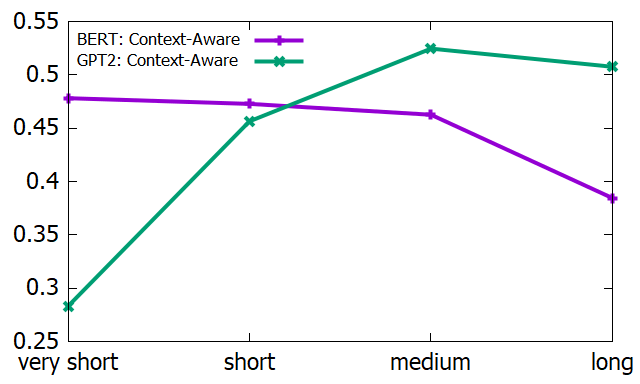
\includegraphics[width=\linewidth]
{./images/new_len_fig.png}}
\caption{\footnotesize \label{fig:length_based} Accuracy for the two context-aware models based on the length of the difficult sentence: very short ($\le 5$ tokens), short ($6-15$), medium ($16-19$), and long ($\ge20$).}
\end{figure}

\begin{figure}[t]
\center{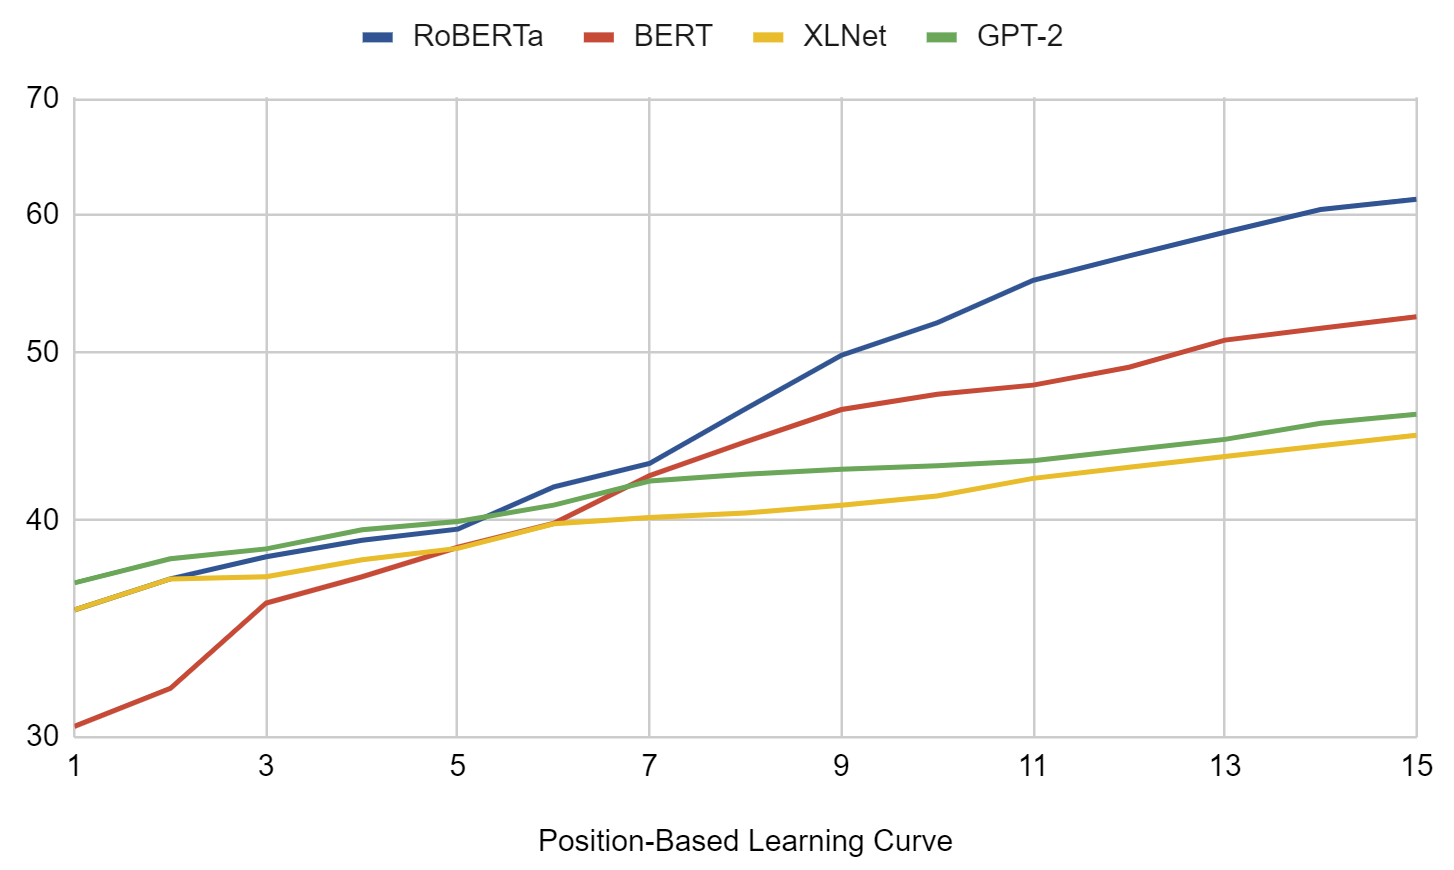
\includegraphics[width=\linewidth]
{./images/new_pos_fig.png}}
\caption{Accuracy for the two context-aware models based on the number of words typed so far ($i$).}
\label{fig:position_based}
\end{figure}

\paragraph{Number of words typed}
Figure \ref{fig:position_based} shows the performance of the two context-aware models based on how many words of the simplification the model has access to, i.e., $i$.  Early on when the sentence is first being developed, both models struggle.  As more and more words are typed and more context is provided, the accuracy of both models increase, however, GPT-2 improves more rapidly as additional context is provided. Like the difficult sentence length analysis, GPT-2 performs better with more context information.

\paragraph{Accuracy@N}

Table \ref{tab:accuracy-@-n} shows the accuracy@N from RoBERTa, BERT, XLNet models on next word prediction. Accuracy@N is a metric that gives a model credit as long as it can provide accurate prediction within its k suggestions. As we can see from here, this relaxing schema helps the models better assist technician because the user can pick the best word in the list of suggestion and therefore can help speed up the process and improve model performance.

\begin{table}[t]
\centering
\scalebox{.9}{%
\begin{tabular}{l c c c c c}
\toprule
 & RoBERTa & BERT & XLNet & \\
 \midrule
accuracy@2 & 67.2 & 54.5 & 46.9 \\
accuracy@3 & 70 & 56.2 & 49.2 \\
accuracy@4 &72.1 & 58.0 & 51.3 \\
accuracy@5 & 73.2 & 59.4 & 53.5 \\
accuracy@6 & 73.2 & 59.4 & 53.5 \\
accuracy@7 & 73.2 & 59.4 & 53.5 \\
 \bottomrule
\end{tabular}}
\caption{\label{tab:accuracy-@-n} Accuracy @ N of the RoBERTa, BERT, and XLNet with context on next word prediction}
\end{table}

\paragraph{Performance on predicting next K words}

Table \ref{tab:next-k-results} show results from four neural network models in predicting the next k words. To further understand how performance affected by the more words it needs to predict, I run experiments with predicting next 1, 2, 3, and 4 words. This idea is the same with the Google email text suggestion when the model suggest multiple words at a time. As more words need to be predicted, the performance drop significantly for the medical domain. This confirms that the task is unsolved and open for researches to further advance the autocompletion system in medical text simplification.

\begin{table}[t]
\centering
\scalebox{.9}{%
\begin{tabular}{l c c c c c}
\toprule
 & RoBERTa & BERT & XLNet & GPT-2 & \\
 \midrule
Next 1 &  62.4 & 53.28 & 46.2 & 49 \\
Next 2 & 45.1 & 38.7 & 33.5 & 41 \\
Next 3 & 36.8 & 31.5 & 26.7 & 31 \\
Next 4 & 31.5 & 24.2 & 21 & 14 \\
 \bottomrule
\end{tabular}}
\caption{\label{tab:next-k-results} Accuracy of the RoBERTa, BERT, XLNet, and GPT-2 with context on next k prediction}
\end{table}

\begin{table}[t]
\centering
\scalebox{.9}{%
\begin{tabular}{l c}
\toprule
 Model & Accuracy \\
 \midrule
Majority Vote & 43.25\% \\
 \midrule
4 Class Classification & 56.45\% \\
 \midrule
Combined Class Classification & 59.3\% \\
 \midrule
AuTS & 64.52\% \\
 \midrule
Upperbound & 66.44\% \\
 \bottomrule
\end{tabular}}
\caption{\label{tab:ensembleResults} Accuracy of the majority vote, 4-class classification, combined class classification, AuTS, and the upperbound of ensemble models.}
\end{table}
%concludes our hypothesis that the further we go along the sentence, the better the prediction of next word from our models. From position 1 to position 10, the performance of BERT increases by 5.9\% (35.53\% to 41.43\%) while GPT-2 gains roughly 15\% (39.43\% to 54.56\%). This observation again confirms our hypothesis that GPT can better capture longer context information; however, in this experiment, in the simplified sentence itself. 

%Another important observation from figure \ref{fig:position_based} is that the improvements decrease as we go further along the simplified sentences. Within the first couple words (see Figure \ref{fig:position_based} position 0 to 4), the improvement is larger as composed to the later positions (position 8 to 10). This observation also suggests that the model can quickly learn the context information and make better prediction. Once again, this concludes that our approach can be used to provide real-time suggestion for TS.   

\section{Conclusions}

In this paper we have introduced a first-of-its-kind medical corpus for text simplification and proposed new task, text simplification with autocompletion.  Unlike most autocomplete tasks, for text simplification, models can be guided by the sentence that the user is simplifying.  We compared four recent PNMLs BERT, RoBERTa, XLNet, and GPT-2, and showed how the difficult sentence could be incorporated into the prediction process. Using context resulted in significant increases in performance with the best model, RoBERTa with context, achieving a prediction accuracy of 62.4\%, getting every other word right. With an intial analysis, we designed the AuTS model, which is an ensemble model that combines adventages of PNLMs and outperforms RoBERTa by 2.1\%. We hope that this new task will allow for other interesting model adaptations to be explored.


%%%%%%%%%%%%%%%End of content%%%%%%%%%%%%%%%
% Added it back on for Sponsor Acknowledgements
%\section*{Acknowledgements}

%The acknowledgements should go immediately before the references.  Do not number the acknowledgements section. Do not include this section when submitting your paper for review.

% include your own bib file like this:
\bibliographystyle{coling}
\bibliography{coling2020}

%\begin{thebibliography}{}

%\bibitem[\protect\citename{Aho and Ullman}1972]{Aho:72}
%Alfred~V. Aho and Jeffrey~D. Ullman.
%\newblock 1972.
%\newblock {\em The Theory of Parsing, Translation and Compiling}, volume~1.
%\newblock Prentice-{Hall}, Englewood Cliffs, NJ.

%\bibitem[\protect\citename{{American Psychological Association}}1983]{APA:83}
%{American Psychological Association}.
%\newblock 1983.
%\newblock {\em Publications Manual}.
%\newblock American Psychological Association, Washington, DC.

%\bibitem[\protect\citename{{Association for Computing Machinery}}1983]{ACM:83}
%{Association for Computing Machinery}.
%\newblock 1983.
%\newblock {\em Computing Reviews}, 24(11):503--512.

%\bibitem[\protect\citename{Chandra \bgroup et al.\egroup }1981]{Chandra:81}
%Ashok~K. Chandra, Dexter~C. Kozen, and Larry~J. Stockmeyer.
%\newblock 1981.
%\newblock Alternation.
%\newblock {\em Journal of the Association for Computing Machinery},
%  28(1):114--133.

%\bibitem[\protect\citename{Gusfield}1997]{Gusfield:97}
%Dan Gusfield.
%\newblock 1997.
%\newblock {\em Algorithms on Strings, Trees and Sequences}.
%\newblock Cambridge University Press, Cambridge, UK.

%\bibitem[\protect\citename{Rasooli and Tetreault}2015]{rasooli-tetrault-2015}
%Mohammad~Sadegh Rasooli and Joel~R. Tetreault. 2015.
%\newblock {Yara parser: {A} fast and accurate dependency parser}.
%\newblock \emph{Computing Research Repository}, arXiv:1503.06733.
%\newblock Version 2.

%\bibitem[\protect\citename{Borschinger and Johnson}2011]{borsch2011}
%Benjamin Borschinger and Mark Johnson. 2011.
%\newblock A particle filter algorithm for {B}ayesian wordsegmentation.
%\newblock In \emph{Proceedings of the Australasian Language Technology Association %Workshop 2011}, pages 10--18, Canberra, Australia.

%\end{thebibliography}

\end{document}
